\subsection{Problem 1: The Sampling Theorem}
\begin{enumerate}
      \item {\bf Analog signals are usually passed through a low-pass filter prior to sampling. Why is this necessary?}

            The low-pass filter is used to remove noise, and to remove frequency components that may be higher than the Nyquist frequency. This is necessary to prevent not accounting for the higher frequency components, which would result in aliasing.

      \item {\bf What is the minimum sampling frequency for a pure sine wave input at 3KHz? Assume that the signal can be completely reconstructed.}

            The minimum sampling frequency for a pure sine wave input at 3KHz would be $f_s > 2 * f_{Nyquist} = 6\text{KHz}$

      \item {\bf What is the Nyquist frequency?}

            The Nyquist frequency is the highest frequency that can be represented in a sampled signal. It is half the sampling frequency and defined as $f_{Nyquist} = \frac{f_s}{2}$

      \item {\bf What are the resulting frequencies for the following input sinusoids 500Hz, 2.5KHz, 5KHz and 5.5KHz if the signals are sampled by a sampling frequency of 5KHz?}

            The frequencies would be:
            \begin{enumerate}
                  \item 500Hz: 500Hz
                  \item 2.5Khz: 0KHz (DC component)
                  \item 5KHz: 0KHz (Aliased)
                  \item 5.5KHz: 0.5KHz (Aliased, by $f - f_{sampling}$)
            \end{enumerate}

      \item {\bf Mention three frequencies of signal that alias to a 7Hz signal. The signal is sampled by a constant 30 Hz sampling frequency.}

            The frequencies would be: $37$Hz, $67$Hz, $97$Hz.
\end{enumerate}

\subsection{Problem 2: Impulse Train Sampling and Real Sampling}

\begin{figure}[H]
      \centering
      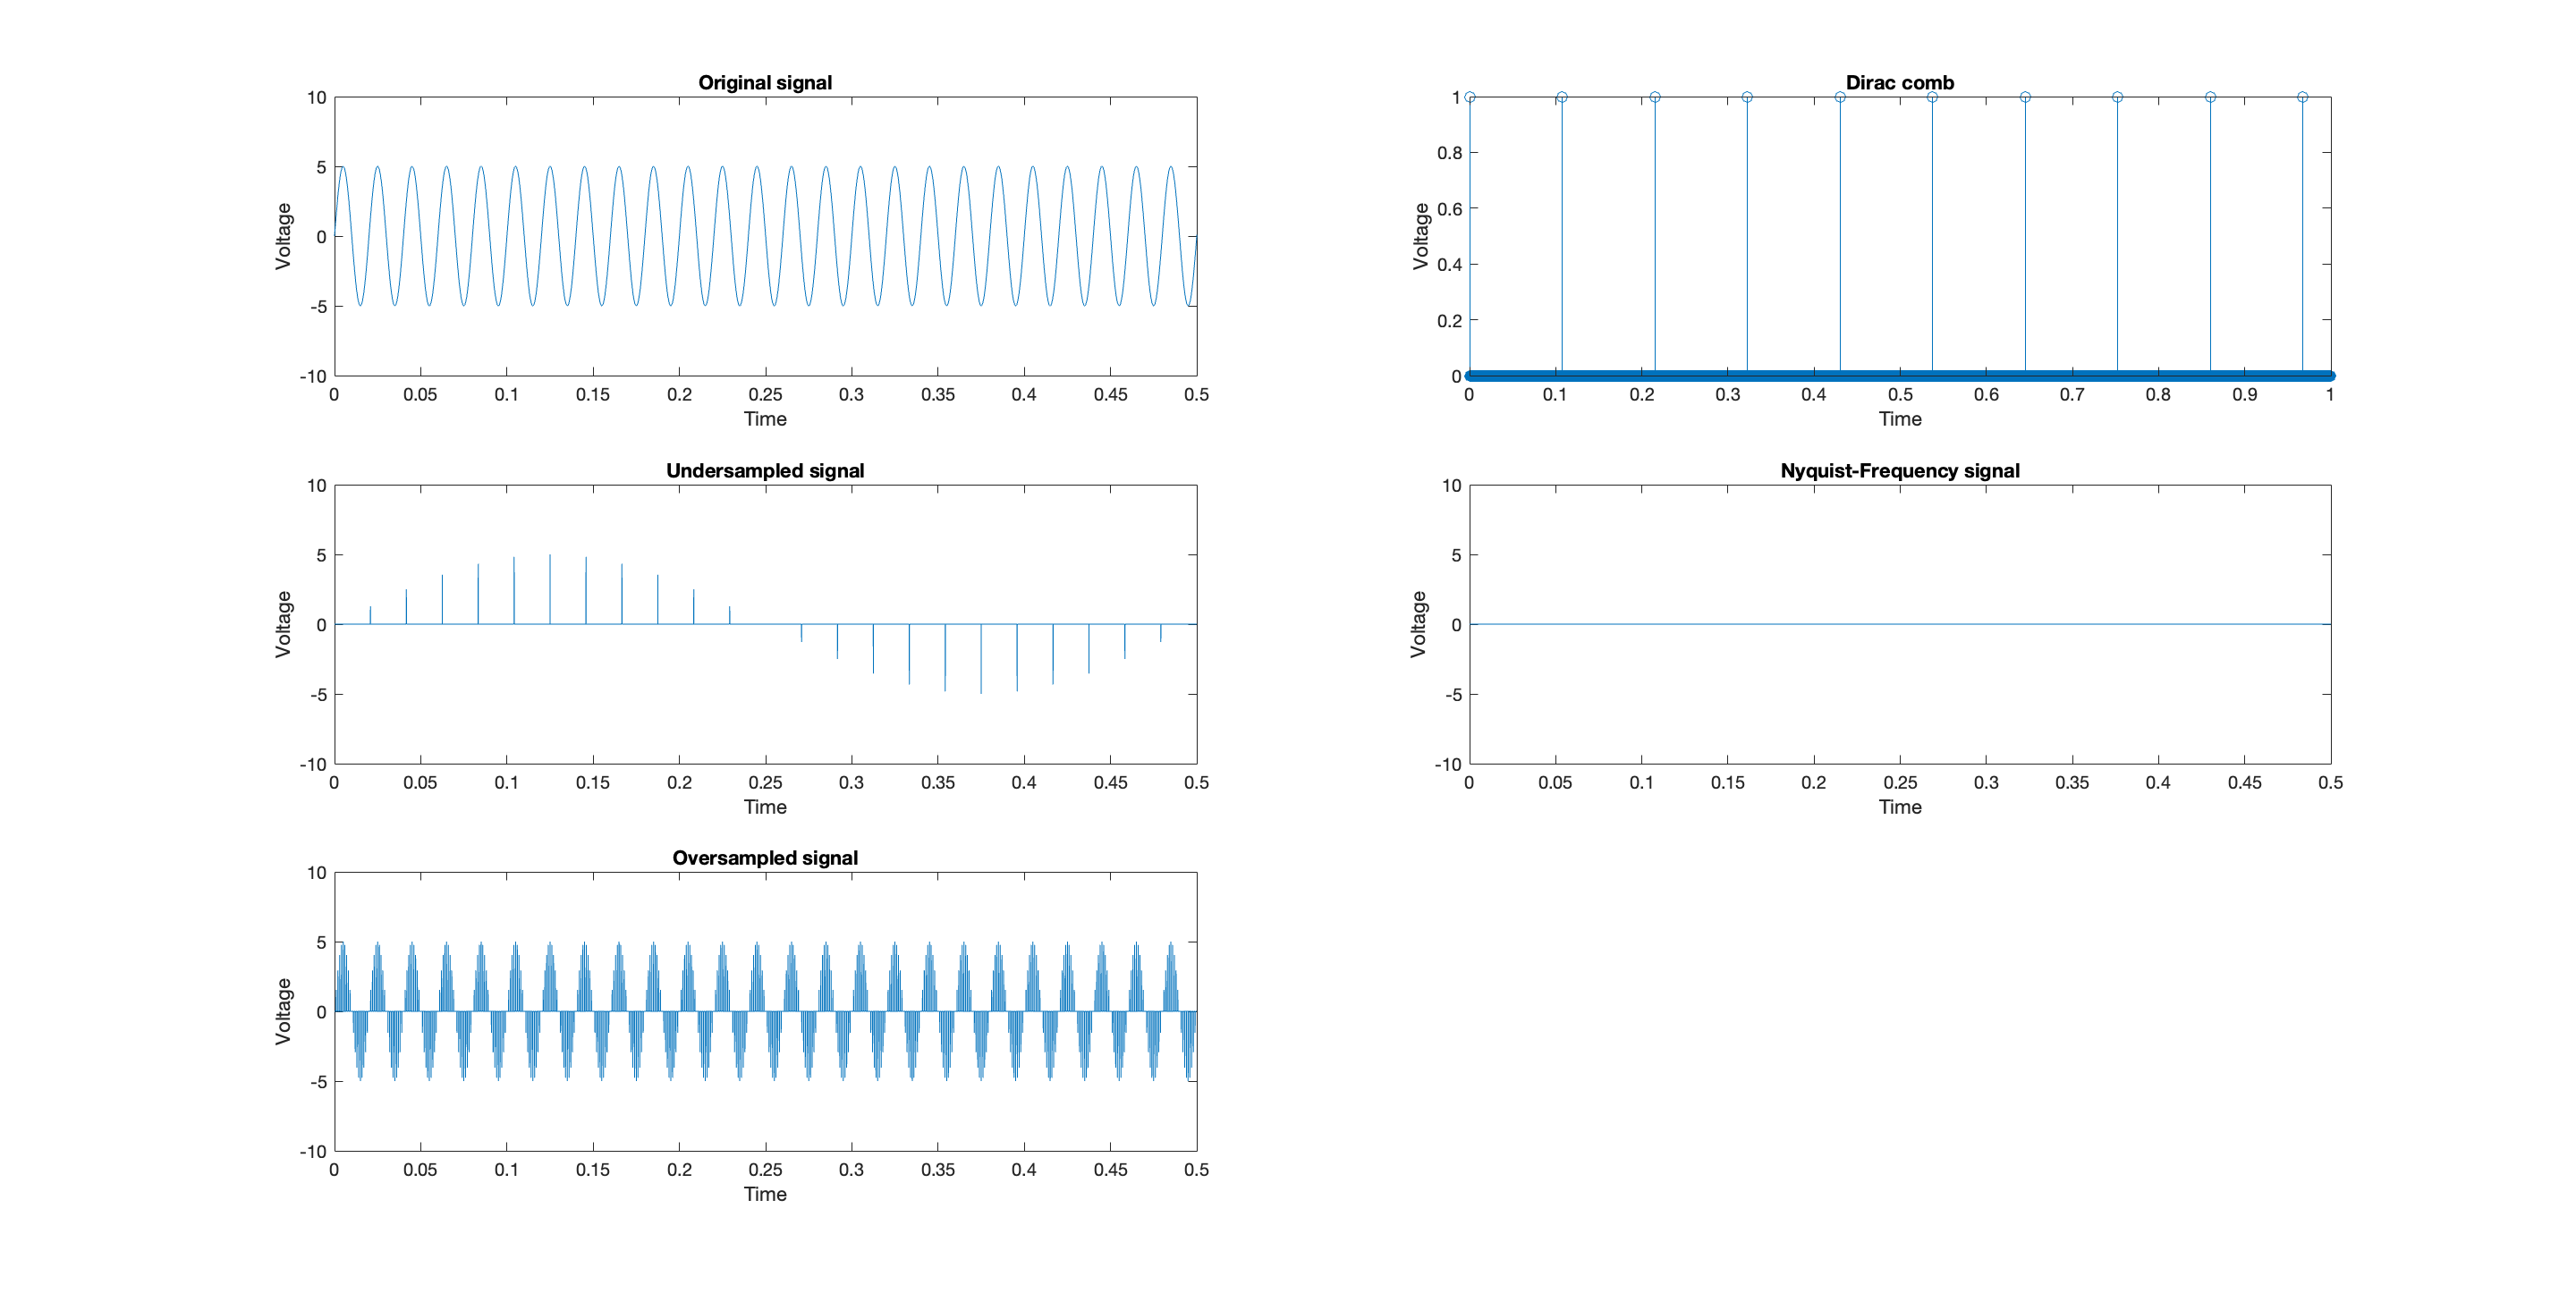
\includegraphics[width=\textwidth]{images/lab_4/problem2_part1.png}
      \caption{Impulse train sampling}
      \label{fig:impulse_train_sampling}
\end{figure}

\begin{figure}[H]
      \centering
      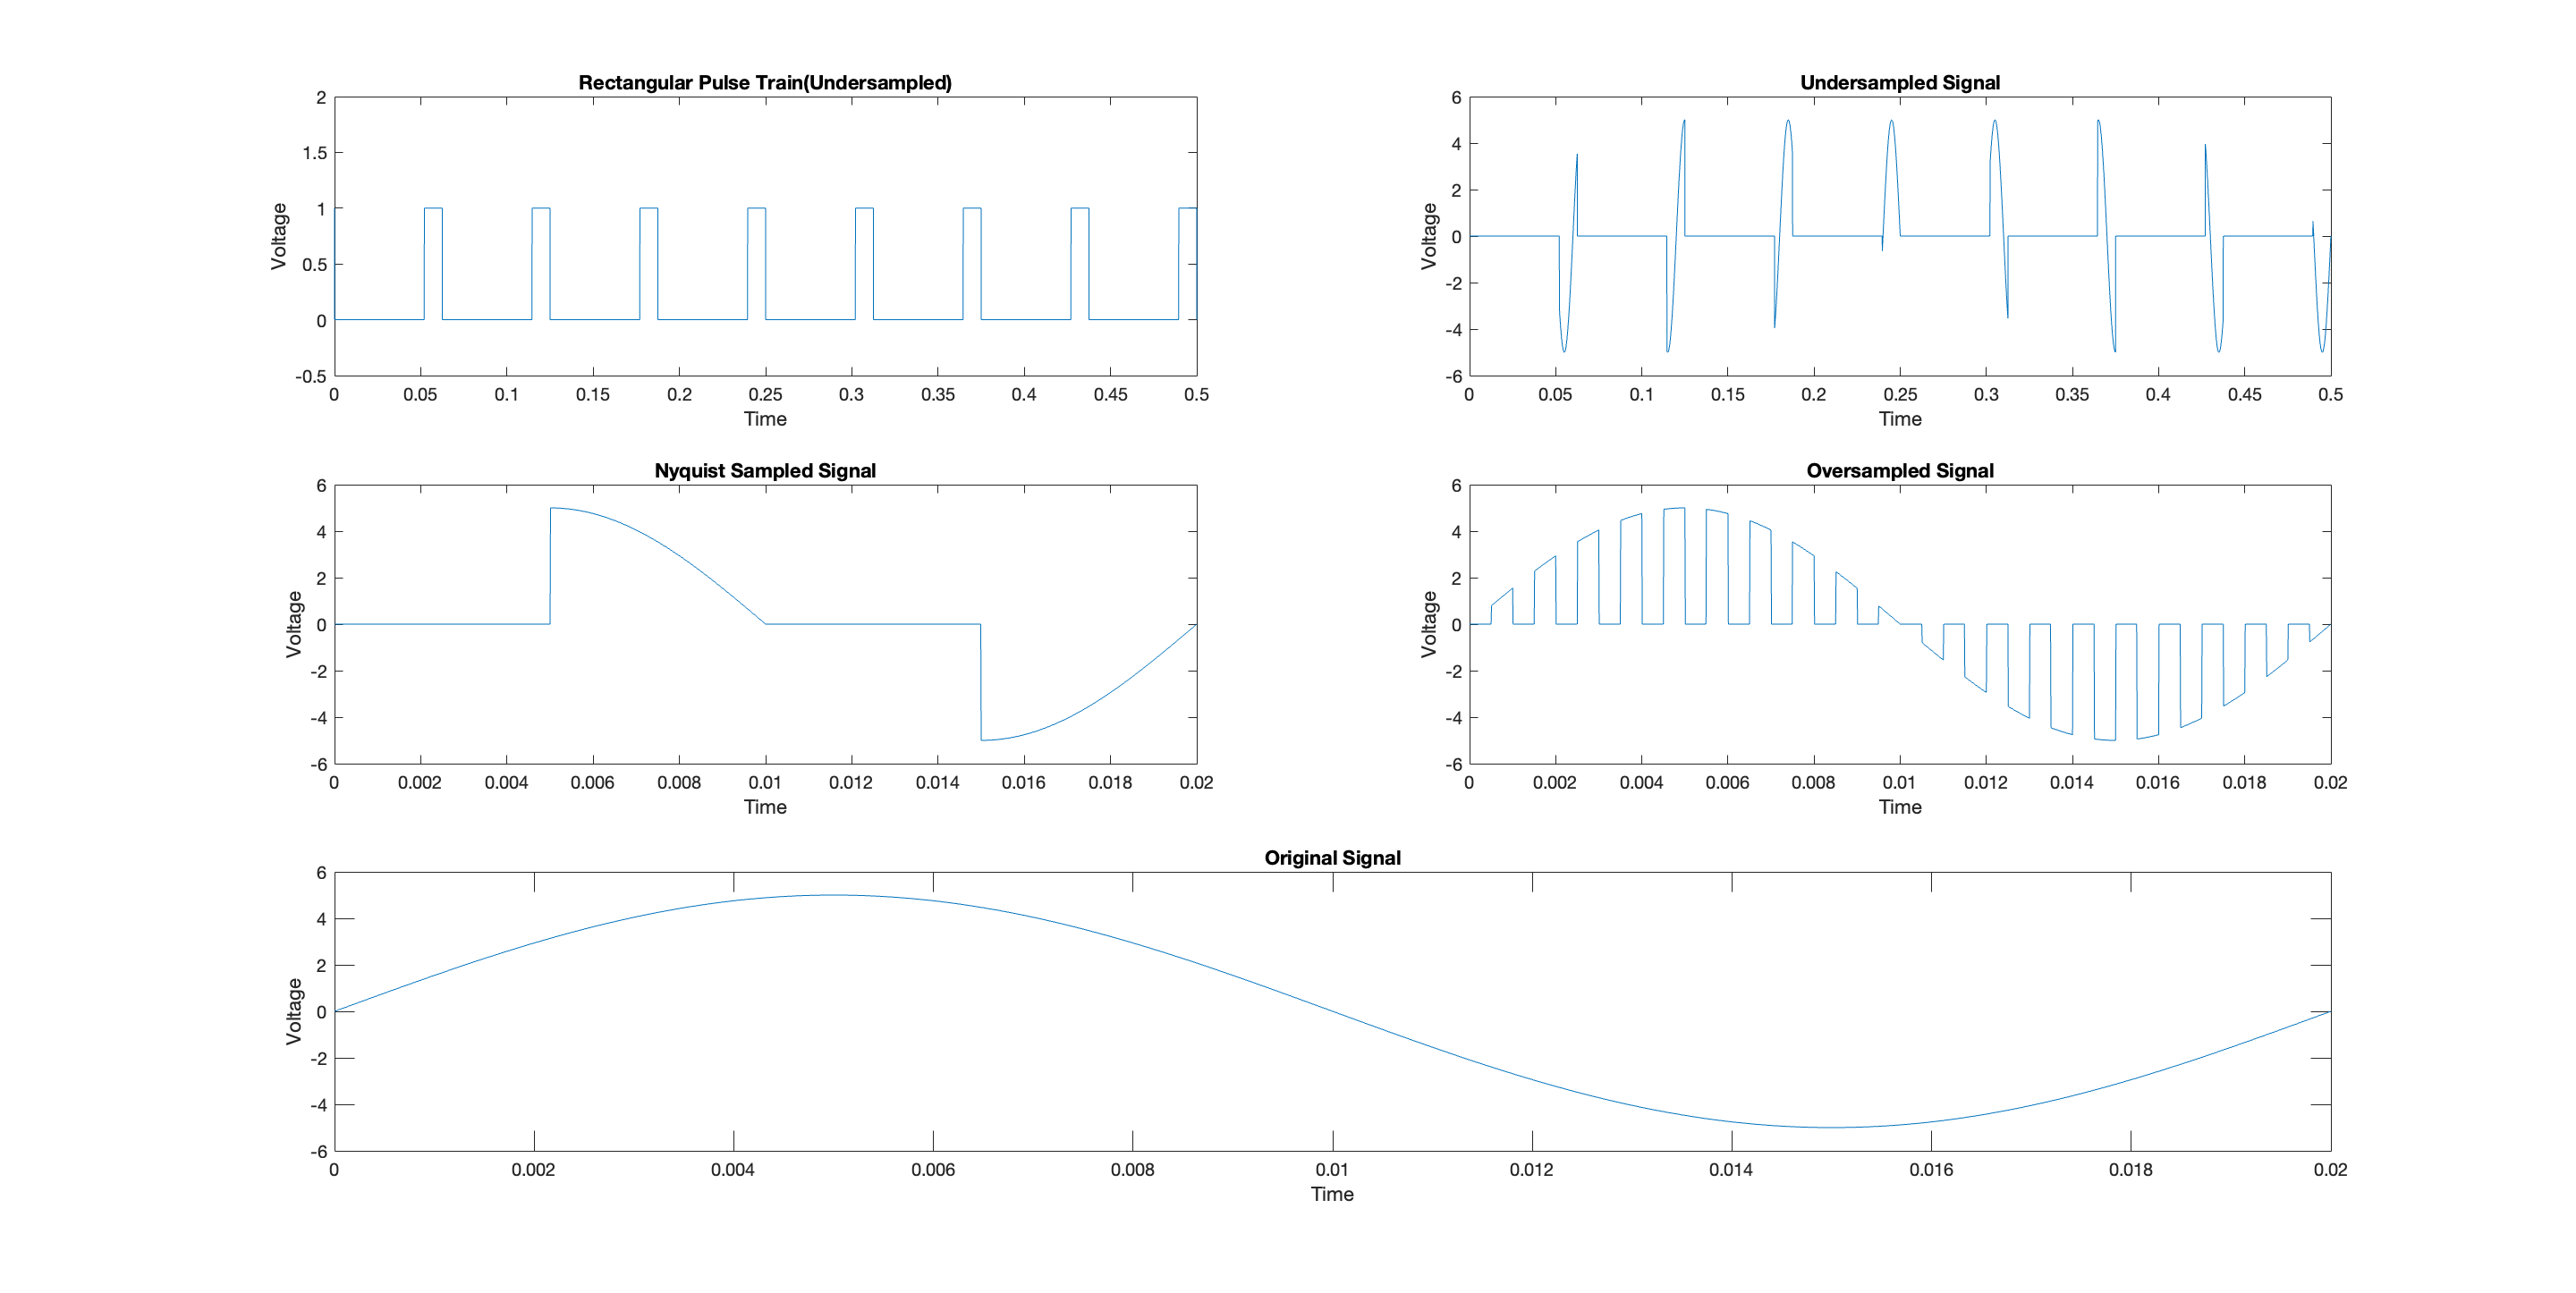
\includegraphics[width=\textwidth]{images/lab_4/problem2_part2.png}
      \caption{Rectangular Pulse Train Sampling}
\end{figure}

The code used to perform the sampling is given below.

\begin{verbatim}
%% Prelab:

% first part:

f = 50; % frequency, in hertz
f_n = 2*f; % nyquist frequency, in hertz

samples=1E5;
t = 0:1/samples:1; % 100kS

V_pp = 5;
w = 2*pi*f;
x = V_pp * sin(w .* t);

% Original signal:
subplot(3, 2, 1);
plot(t, x);
ylabel("Voltage")
xlabel("Time")
title("Original signal");
ylim([-10, 10]);
xlim([0, 0.5]);

% Dirac comb
subplot(3, 2, 2);
p = zeros(size(t));
p(1:10750:length(t)) = 1;
stem(t, p);
ylabel("Voltage")
xlabel("Time")
title("Dirac comb");
ylim([0, 1]);
xlim([0, 1]);

% Undersampled signal:
fs = 48; % In hertz

p = zeros(size(t));
p(1:samples/fs:length(t)) = 1;

subplot(3, 2, 3);
plot(t, p .* x);
ylabel("Voltage")
xlabel("Time")
title("Undersampled signal");
ylim([-10, 10]);
xlim([0, 0.5]);

% Nyquist-Frequency sampled signal
fs = 100; % In hertz

p = zeros(size(t));
p(1:samples/fs:length(t)) = 1;

subplot(3, 2, 4);
plot(t, p .* x);
ylabel("Voltage")
xlabel("Time")
title("Nyquist-Frequency signal");

ylim([-10, 10]);
xlim([0, 0.5]);

% Oversampled signal
fs = 1000; % In hertz

p = zeros(size(t));
p(1:samples/fs:length(t)) = 1;

subplot(3, 2, 5);
plot(t, p .* x);
ylabel("Voltage")
xlabel("Time")
title("Oversampled signal");

ylim([-10, 10]);
xlim([0, 0.5]);

%%

clear
close all

f = 50;
t = 0:1E-5:1;
V_pp = 5;
w = 2*pi*f;
x = V_pp * sin(w .* t);

% Underdamped signal:
fs = 48; % In hertz
T = 1/fs;
T0 = 0.5 * 1/fs;
p = gen_pulse_train(t, T0, T);

subplot(3, 2, 1);
plot(t, p);
title("Rectangular Pulse Train(Undersampled)");
ylabel("Voltage")
xlabel("Time")
xlim([0, 1/2]);
ylim([-0.5, 2]);

subplot(3, 2, 2);
plot(t, p .* x);
ylabel("Voltage")
xlabel("Time")
title("Undersampled Signal")
xlim([0, 1/2]);
ylim([-6, 6]);


% Nyquist Sampled signal:
fs = 100; % In hertz
T = 1/fs;
T0 = 0.5 * 1/fs;
p = gen_pulse_train(t, T0, T);

subplot(3, 2, 3);
plot(t, p .* x);
ylabel("Voltage")
xlabel("Time")
title("Nyquist Sampled Signal")
xlim([0, 1/50]);
ylim([-6, 6]);

% Overly Sampled signal:
fs = 1000; % In hertz
T = 1/fs;
T0 = 0.5 * 1/fs;
p = gen_pulse_train(t, T0, T);

subplot(3, 2, 4);
plot(t, p .* x);
ylabel("Voltage")
xlabel("Time")
title("Oversampled Signal")
xlim([0, 1/50]);
ylim([-6, 6]);

subplot(3, 2, [5 6]);
plot(t, x);
ylabel("Voltage")
xlabel("Time")
title("Original Signal")
xlim([0, 1/50]);
ylim([-6, 6]);

% Function to generate pulse train
function [p] = gen_pulse_train(t, T0, T)
      p = zeros(size(t));
      for k=1:length(t)
            if mod(t(k), T) == 0
            left = t(k) - T0;
            right = t(k) + T0;
            p((t > left) & (t < right)) = 1;
            else
            p(k) = 0;
            end
      end
end      
\end{verbatim}
\newpage
\subsection{Problem 3: Sampling using a Sampling bridge}
\begin{figure}[H]
      \centering
      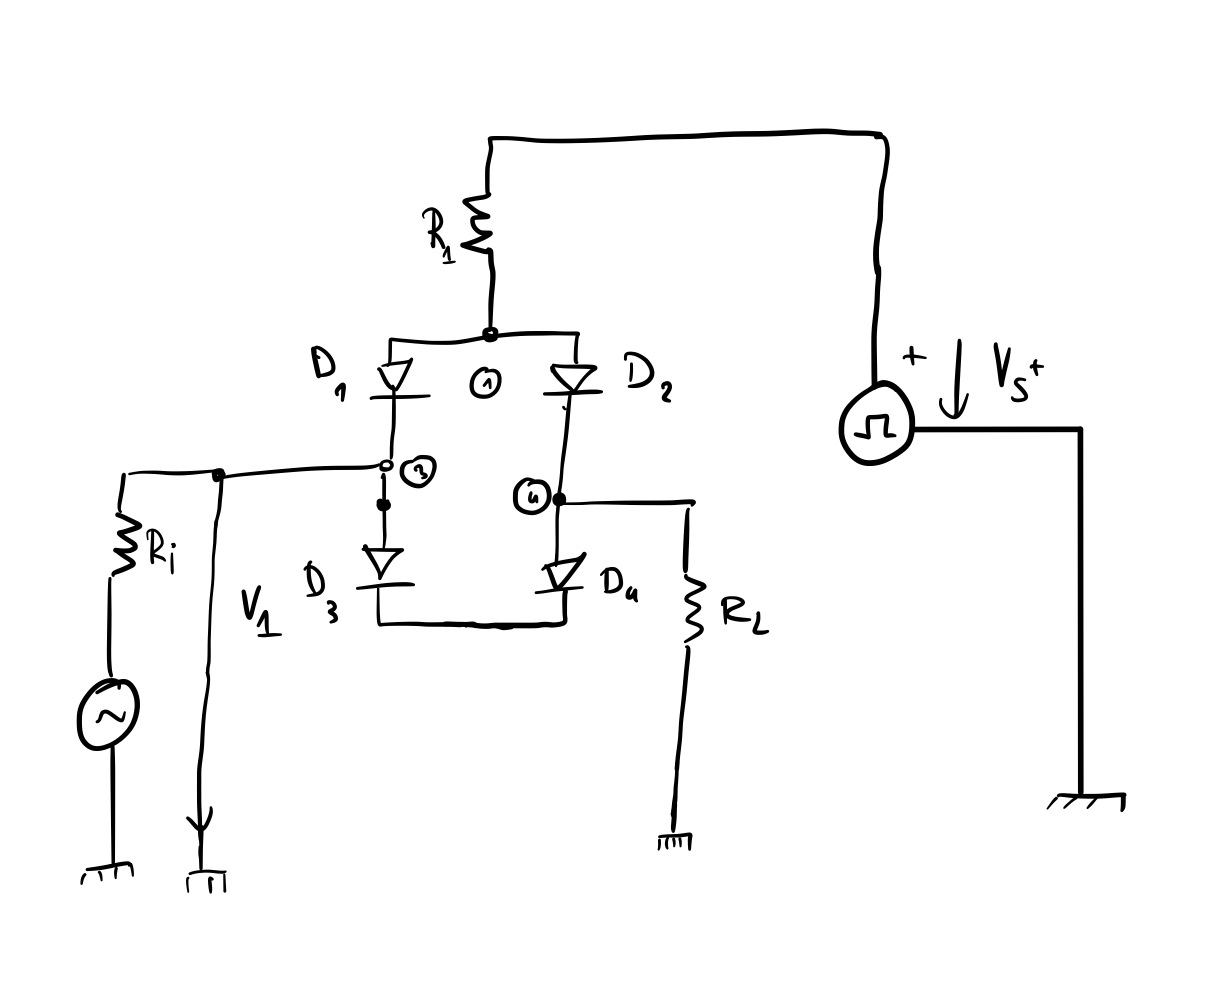
\includegraphics[width=\textwidth]{images/lab_4/problem3_circuit.jpeg}
      \caption{The modified Sampling Bridge circuit.}
\end{figure}

The reason this sampling bridge circuit works is due to the polarity of the two different voltage sources given in the original circuit being practically the same, with the potential being the same for both sources, we can simply omit one and lead current into the same square wave generator.